%!TEX root = kotov.tex
\section{Task 3}
\begin{task}
    Про поиск ближайших $k$ элементов к медиане
    \begin{enumerate}[(a)]
        \item по индексу
        \item по модулю разности значений
    \end{enumerate}
\end{task}

\begin{solution}
    \begin{enumerate}[(a)]
        \item
        За линейные времена найдем медиану $m$ и, например, $m-k/2$ статистику.
        \begin{remark}
            Где надо, там правильно округляем до целого.
        \end{remark}
        Затем, выкинем левую часть исходного массива, то есть ту часть, элементы в которой меньше, чем найденная статистика
        \begin{figure}[H]
            \centering
            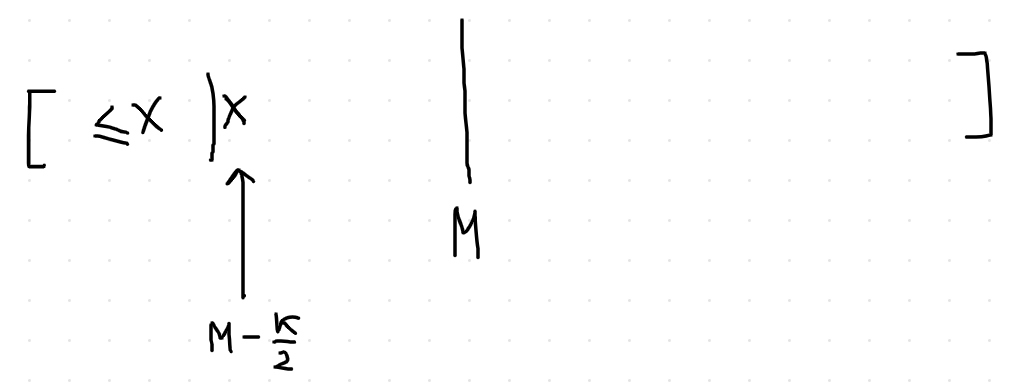
\includegraphics[scale=0.3]{pics/3_1.png}
            \caption{Художественная картинка, поясняющая слова}
        \end{figure}
        и будем рассматривать оставшуюся часть массива. Найдем в ней $k$-ую статистику (она соответствует $m+k/2$-ой статистике исходного массива). В ответ выводим элементы, от начала до найденной последней статистике.
        \item
        Сначала также найдем медиану $m$. Теперь создадим новый массив $b$, значения элементов которого $b_i = |a_i - m|$, где $a$ --- исходный массив. Эти все действия мы делали за $\O(n)$.
        
        Теперь в массиве $b$ найдем $k$-ую порядковую статистику (обозначим ее за $y$), тогда в массиве слева будет блок, элементы которого будут $< y$, берем в ответ начало этого массива до найденной $k$-ой порядковой статистики.
        \begin{remark}
            Имеется в виду, что мы запоминаем в пару индекс элементов из исходного массива, чтобы можно было потом легко восстановить значения самих элементов
        \end{remark}
        \begin{remark}
            Так как к этому моменту в массиве $b_i$ хранится ``расстояние'' элементов до медианы, то $k$-ая порядковая статистка в таком массиве говорит нам, какой элемент находится $k$-ым по счету по ``расстоянию'' до медианы.
        \end{remark}
    \end{enumerate}
\end{solution}